%\documentclass[tikz,convert={outfile=\s1.svg}]{standalone}
\documentclass[tikz]{standalone}
\usepackage{amsthm}
\usepackage[landscape]{geometry}
\usepackage{multicol}
\usepackage{tikz}
\usepackage{pgfplots}
\usepackage{xcolor}
\usepackage{amsmath}
\usepackage[T1]{fontenc}
\usepackage{utopia}
\usepackage{changepage}
\usepackage{amssymb}
\usepackage{fancyhdr}
\usepackage[many]{tcolorbox}
\usepackage{moresize}
\usepackage{fullpage}
\usepackage{mathpazo}
\usepackage{tikz-3dplot}
\usepackage{cancel}
\tdplotsetmaincoords{70}{165}
\pgfplotsset{compat=1.18}
\usepackage{enumitem}
\usepackage{tabularray}
\usepackage{mathtools}

\UseTblrLibrary{diagbox}

\usetikzlibrary{
    shadings, calc, patterns, angles, quotes, arrows.meta, 
    decorations.pathmorphing, decorations.pathreplacing, 
    fadings, 3d, perspective, backgrounds, intersections, 
    decorations.markings, bending, positioning, 							spy,shapes.geometric,shadows,shapes.symbols, fadings, matrix, fit
}

\usepgfplotslibrary{
    groupplots, external, colormaps, patchplots, fillbetween
}


% Reds (r)
\definecolor{r1}{RGB}{255, 191, 191}    % Light coral
\definecolor{r2}{RGB}{255, 191, 223}    % Light pink
\definecolor{r3}{RGB}{255, 207, 207}    % Light rose

% Blues (b)
\definecolor{b1}{RGB}{191, 223, 255}    % Light blue
\definecolor{b2}{RGB}{191, 239, 255}    % Light sky
\definecolor{b3}{RGB}{191, 255, 255}    % Light cyan

% Greens (g)
\definecolor{g1}{RGB}{191, 255, 191}    % Light green
\definecolor{g2}{RGB}{191, 255, 223}    % Light mint
\definecolor{g3}{RGB}{207, 255, 207}    % Light sage

% Oranges (o)
\definecolor{o1}{RGB}{255, 223, 191}    % Light peach
\definecolor{o2}{RGB}{255, 239, 191}    % Light cream
\definecolor{o3}{RGB}{255, 231, 191}    % Light buff

% Violets (v)
\definecolor{v1}{RGB}{223, 191, 255}    % Light purple
\definecolor{v2}{RGB}{239, 191, 255}    % Light lilac
\definecolor{v3}{RGB}{231, 191, 255}    % Light lavender

% Yellows (y)
\definecolor{y1}{RGB}{255, 255, 191}    % Light yellow
\definecolor{y2}{RGB}{255, 247, 191}    % Light cream yellow
\definecolor{y3}{RGB}{255, 239, 191}    % Light warm cream

\definecolor{w}{HTML}{eeeeee}
\definecolor{g}{HTML}{444444}
\definecolor{b}{HTML}{222222}
\definecolor{lightgrey}{HTML}{cccccc}
\definecolor{firebrick}{RGB}{178, 34, 34}
\definecolor{myg}{RGB}{3, 252, 177}


\color{w}
\begin{document}
\ssmall
%\pagecolor{b}
\nopagecolor
\fontfamily{put}

		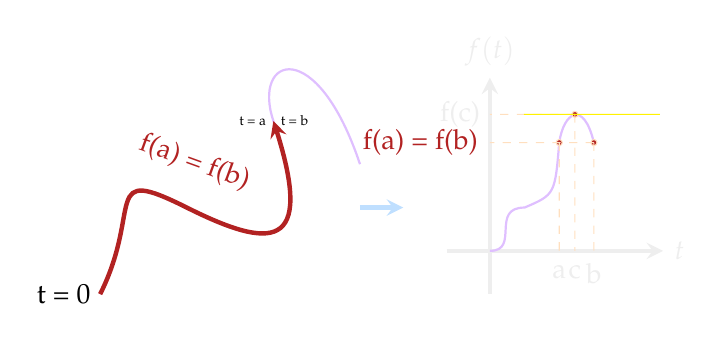
\begin{tikzpicture}[scale=0.55]
			\coordinate (c1) at (-5, -1);
			\coordinate (c2) at (-3, 1);
			\coordinate (c3) at (-1, 3);
			\coordinate (c4) at (1, 2);
			
			\coordinate (b1) at	($(c1) + (1, 2)$);
			
			\coordinate (b21) at ($(c2) + (-2, 1)$);
			\coordinate (b22) at ($(b21)!2!(c2)$);
			
			\coordinate (b31) at ($(c3) + (1, -3)$);
			\coordinate (b32) at ($(b31)!1.5!(c3)$);
			
			\coordinate (b41) at ($(c4) + (-1, 3)$);
			
			\draw[draw=v1, thick] (c1) .. controls (b1) and (b21) .. (c2)
				.. controls (b22) and (b31) .. (c3)
				.. controls (b32) and (b41) .. (c4);
				
			\node[left] at (c1) {t = 0};
			\node[left, outer sep=2pt, scale=0.5] at (c3) {t = a};
			\node[right, outer sep=2pt, scale=0.5] at (c3) {t = b};		
			
			\node[above=3mm, rotate = -20, text=firebrick] at (c2) {f(a) = f(b)}; 
			
			\draw[draw=firebrick, ultra thick, -stealth] (c1) .. controls (b1) and (b21) .. (c2)
				.. controls (b22) and (b31) .. (c3)	;
			
			\draw[draw=w, ultra thick, -stealth] (3, 0) -- (8, 0) node[text=w, right] {$t$};
			\draw[draw=w, ultra thick, -stealth] (4, -1) -- (4, 4) node[text=w, above] {$f(t)$};
				
			\draw[ultra thick, -stealth, b1] (1, 1) -- (2, 1);		
				
				
			\coordinate (o) at (4, 0);		
			
			\def\r{0.4}			
			
 			\coordinate (f1) at (o);
 			\coordinate (f2) at ($(o) + (\r*2, 1)$);
 			\coordinate (f3) at ($(o) + (\r*4, 2.5)$);
 			\coordinate (f4) at ($(o) + (\r*6, 2.5)$);
 			\coordinate (f5) at ($(o) + (\r*8, 1)$);
 			
 			
 			\coordinate (f11) at ($(f1) + (0.7, 0)$);
 			
 			\coordinate (f21) at (f2 -| o);
 			\coordinate (f22) at ($(f2) + (0.7, 0.3)$);
 			
 			\coordinate (f31) at ($(f3) + (-1, 0)$);
 			\coordinate (f32) at ($(f3) + (0.1, 0.7)$);
 			
 			\coordinate (f41) at ($(f3)!0.7!(f4) + (0, 1)$);
 			
 			\draw[draw=v1, thick] (f1) .. controls (f11) and (f21) .. (f2)
				.. controls (f22) .. (f3)
				.. controls (f32) and (f41) .. (f4);
				
				
				
			\coordinate (A) at (f3);
			\coordinate (B) at (f4);
			\coordinate (C) at ($(A)!0.45!(B) + (0, 0.65)$);
			
			\filldraw[draw=o1, fill=firebrick] (A) circle (2pt);
			\filldraw[draw=o1, fill=firebrick] (B) circle (2pt);
			\filldraw[draw=o1, fill=firebrick] (C) circle (2pt);
			
			\coordinate (Ax) at (A |- o);
			\coordinate (Ay) at (A -| o);
			
			\coordinate (Bx) at (B |- o);
			\coordinate (By) at (B -| o);
			
			\coordinate (Cx) at (C |- o);
			\coordinate (Cy) at (C -| o);			
			
			\draw[dashed, draw=o1] (A) -- (Ax)	;
%			\draw[dashed, draw=o1] (A) -- (Ay)	;
			
			\draw[dashed, draw=o1] (B) -- (Bx)	;
			\draw[dashed, draw=o1] (B) -- (By)	;

			\draw[dashed, draw=o1] (C) -- (Cx)	;
			\draw[dashed, draw=o1] (C) -- (Cy)	;
			
			
			\node[below, text=w, outer sep =2pt] at (Ax) {a};
			\node[below, text=w, outer sep =1pt] at (Bx) {b};
			\node[below, text=w, outer sep =2pt] at (Cx) {c};
			\node[left, outer sep=1pt] at (Ay) {\textcolor{firebrick}{f(a) = f(b)}};
			\node[left, text=w] at (Cy) {f(c)};	
			
			\draw[draw=yellow] ($(Cy)!0.4!(C)$) -- ($(Cy)!2!(C)$);
			
		\end{tikzpicture}

\end{document}